\documentclass[tikz, border=2pt]{standalone}
\usepackage{amsmath}

\begin{document}
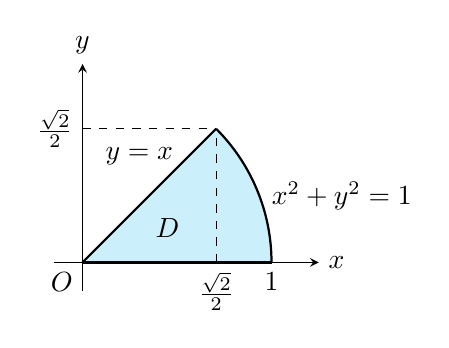
\begin{tikzpicture}[scale=2.4, >=stealth]
  % D: 0 <= r <= 1, 0 <= theta <= pi/4
  \fill[cyan!20] (0,0) -- (1,0) arc[start angle=0,end angle=45,radius=1] -- cycle;

  \draw[->] (-0.15,0) -- (1.25,0) node[right] {$x$};
  \draw[->] (0,-0.15) -- (0,1.05) node[above] {$y$};

  \draw[thick] (0,0) -- (1,0);
  \draw[thick] (0,0) -- ({sqrt(2)/2},{sqrt(2)/2});
  \draw[thick] (1,0) arc[start angle=0,end angle=45,radius=1];
  \draw[dashed] ({sqrt(2)/2},0) -- ({sqrt(2)/2},{sqrt(2)/2});
  \draw[dashed] (0,{sqrt(2)/2}) -- ({sqrt(2)/2},{sqrt(2)/2});

  \node[below left] at (0,0) {$O$};
  \node[below] at (1,0) {$1$};
  \node[below] at ({sqrt(2)/2},0) {$\frac{\sqrt2}{2}$};
  \node[left] at (0,{sqrt(2)/2}) {$\frac{\sqrt2}{2}$};
  \node at (0.45,0.18) {$D$};
  \node at (0.3,0.56) {$y=x$};
  \node[right] at (0.95,0.35) {$x^2+y^2=1$};
\end{tikzpicture}
\end{document}
